% NeurIPS 2026 submission
% Prompt Fragility in TruthfulQA
\documentclass{article}

% NeurIPS style
\usepackage[final]{neurips_2025}  % use [preprint] for arXiv, [final] for camera-ready

\usepackage[utf8]{inputenc}
\usepackage[T1]{fontenc}
\usepackage{hyperref}
\usepackage{url}
\usepackage{booktabs}
\usepackage{amsfonts}
\usepackage{amsmath}
\usepackage{nicefrac}
\usepackage{microtype}
\usepackage{xcolor}
\usepackage{graphicx}
\usepackage{subcaption}
\usepackage{multirow}
\usepackage{array}
\usepackage{enumitem}

% Custom commands
\newcommand{\psi}{\text{PSI}}
\newcommand{\tval}{\tau}
\newcommand{\todo}[1]{\textcolor{red}{[TODO: #1]}}
\newcommand{\result}[1]{\textcolor{blue}{\textbf{[#1]}}}

\title{Prompt Fragility in TruthfulQA: Stability of Accuracy and Model Rankings Under Benign Perturbations}

\author{
  Nicholas E. Johnson \\
  \texttt{nicholas.e.johnson@stonybrook.edu} \\  % TODO: update
  %% \And
  %% Co-author \\
  %% Affiliation \\
}

\begin{document}

\maketitle

% ============================================================================
% ABSTRACT
% ============================================================================
\begin{abstract}
Large language model (LLM) benchmarks are typically reported as single accuracy scores, yet the prompt used to elicit answers is a free variable that is rarely varied systematically.
We measure the sensitivity of TruthfulQA multiple-choice (MC1) accuracy to benign prompt perturbations across eight open-source instruction-tuned LLMs spanning three model families and two orders of magnitude in parameter count (3B--72B).
Using 13 prompt conditions---spanning instruction wording, answer formatting, benign distractors, social style, and a constrained chain-of-thought variant---we quantify both per-model accuracy instability and cross-model ranking instability.
We introduce the \emph{Prompt Sensitivity Index} (PSI), defined as the gap between a model's baseline and worst-case accuracy across prompt conditions, and report paired bootstrap confidence intervals for all condition-level deltas.
Our results show that \result{prompt wording alone can shift MC1 accuracy by up to XX percentage points, and the top-ranked model changes in Y out of 13 conditions}.
These findings demonstrate that single-prompt benchmark evaluations substantially understate measurement uncertainty and can produce misleading model comparisons.
We release our full evaluation framework, prompt conditions, and per-prediction logs to support reproducible prompt sensitivity auditing.
\end{abstract}

% ============================================================================
% 1. INTRODUCTION
% ============================================================================
\section{Introduction}
\label{sec:intro}

LLM benchmarks such as MMLU~\citep{hendrycks2021measuring}, HellaSwag~\citep{zellers2019hellaswag}, and TruthfulQA~\citep{lin2022truthfulqa} are central to how the research community and industry practitioners compare model capabilities.
Leaderboard positions, model cards, and deployment decisions frequently hinge on single-point accuracy estimates derived from a fixed prompt template.
Yet the prompt itself---the system instruction, answer format, label scheme, and surrounding context---is a design choice that is rarely subjected to systematic sensitivity analysis.

This is problematic because recent work has shown that LLMs can be surprisingly sensitive to superficial prompt features.
\citet{sclar2024quantifying} demonstrated that minor formatting changes (e.g., separator characters, spacing, casing) can shift few-shot accuracy by up to 76 percentage points.
\citet{mizrahi2024state} evaluated 20 LLMs across 39 tasks with paraphrased instructions and found that different templates lead to substantially different absolute and relative performance, undermining single-prompt comparisons.
If benchmark scores are not stable under benign prompt variation, they are not reliable measurements---they are point samples from an unknown distribution over prompt space.

We focus on TruthfulQA~\citep{lin2022truthfulqa}, a widely used benchmark for assessing factual accuracy and resistance to common misconceptions.
Its multiple-choice (MC1) format---where the model must select a single correct answer from several options---should in principle be more robust to prompt variation than open-ended generation, since the task structure constrains the output space.
We test whether this expectation holds.

Specifically, we address three research questions:
\begin{enumerate}[leftmargin=*, label=\textbf{RQ\arabic*}]
    \item How much does MC1 accuracy vary under semantically equivalent prompt changes?
    \item Which categories of perturbation (instruction wording, formatting, distractors, social style, constrained reasoning) cause the largest accuracy shifts?
    \item Do model rankings remain stable across prompt variants, or do benign changes alter which model appears ``best''?
\end{enumerate}

To answer these questions, we design 13 prompt conditions (1 baseline + 12 perturbations organized into 5 categories) and evaluate 8 instruction-tuned LLMs from the Qwen, Llama, Mistral, Gemma, and Phi families, spanning 3B to 72B parameters.
All conditions are \emph{semantically equivalent}: they present the same question, the same answer choices, and the same correct answer.
They differ only in instruction phrasing, label format, surrounding context, or stylistic tone.

We introduce the \textbf{Prompt Sensitivity Index (PSI)}, a simple metric that captures the gap between baseline and worst-case accuracy for a given model.
Unlike aggregate robustness measures, PSI is directly interpretable: it tells a practitioner how much their reported score could drop under an equally valid prompt.
We complement PSI with ranking stability metrics---Kendall's $\tau$, pairwise rank flip rate, and top-1 instability---to characterize how prompt variation affects not just absolute accuracy but the relative ordering of models.

All experiments use deterministic decoding (\texttt{temperature=0}, \texttt{do\_sample=False}) with fixed random seeds, and we report paired bootstrap confidence intervals (10,000 resamples) for every condition delta.
Our evaluation framework, prompt conditions, and full per-prediction logs are publicly available to support reproducible prompt sensitivity auditing.\footnote{Code and data: \url{https://github.com/ANONYMIZED}}


% ============================================================================
% 2. RELATED WORK
% ============================================================================
\section{Related Work}
\label{sec:related}

\paragraph{Prompt sensitivity in LLM evaluation.}
The observation that LLMs are sensitive to prompt phrasing has been documented across multiple evaluation settings.
\citet{sclar2024quantifying} conducted a systematic study of prompt formatting effects in few-shot settings, finding that surface-level features such as separator tokens, whitespace, and label ordering can cause accuracy swings of up to 76 points.
They proposed FormatSpread, an algorithm for estimating the performance interval across plausible prompt formats without requiring access to model weights.
\citet{mizrahi2024state} scaled this analysis to 20 LLMs and 39 tasks using instruction paraphrases, confirming that single-prompt evaluations can misrepresent both absolute and relative model performance.
They proposed multi-prompt metrics tailored to different evaluation use cases (model development vs.\ downstream deployment).

More recently, \citet{voronov2024mind} investigated prompt sensitivity specifically in multiple-choice benchmarks and showed that option ordering, label schemes, and instruction phrasing all contribute to measurement variance.
\citet{wang2024prosa} introduced ProSA, a framework incorporating PromptSensiScore---a metric based on decoding confidence---to assess and explain prompt sensitivity, finding that larger models tend to exhibit greater robustness but that sensitivity varies substantially across tasks.
\citet{zheng2024prompt} examined prompt robustness in the context of LLM-as-judge evaluation, finding that judge models themselves exhibit significant sensitivity to prompt variation.

Our work extends this line of research in several ways: we focus specifically on TruthfulQA, which tests factual accuracy rather than general language understanding; we evaluate current-generation instruction-tuned models (2024--2025 releases) at scales from 3B to 72B; and we introduce PSI as a practical metric for reporting prompt sensitivity alongside benchmark scores.

\paragraph{TruthfulQA and factual accuracy benchmarks.}
TruthfulQA~\citep{lin2022truthfulqa} was designed to measure whether models generate truthful answers to questions where common misconceptions might lead to errors.
The benchmark comprises 817 questions spanning 38 categories, with both open-ended generation and multiple-choice (MC1/MC2) evaluation modes.
A notable finding from the original paper was an inverse scaling trend: larger models were more likely to produce persuasive but false answers, possibly because they more effectively learn and reproduce human misconceptions from training data.

TruthfulQA is widely used in model cards, leaderboards, and safety evaluations, making the stability of its scores practically important.
However, the benchmark was designed with a single default prompt, and the MC evaluation protocol does not specify how sensitive results are to prompt variation.
Our study fills this gap by systematically characterizing MC1 score variability under controlled perturbations.

\paragraph{Benchmark robustness and leaderboard reliability.}
Beyond prompt sensitivity, several studies have questioned the reliability of LLM benchmarks more broadly.
\citet{alzahrani2024benchmarks} showed that data contamination can inflate benchmark scores, with some model families exhibiting up to 13\% accuracy drops on decontaminated test sets.
\citet{polo2024tinybenchmarks} proposed efficient benchmark subsets (TinyBenchmarks) and found that benchmark agreement---measured by Kendall's $\tau$ between different benchmark rankings---is often lower than assumed, particularly when restricting to top-performing models.
\citet{zhu2024benchbench} introduced a meta-evaluation framework (BenchBench) showing that conclusions about benchmark reliability are themselves sensitive to methodological choices such as model sampling and correlation metrics.

These findings collectively suggest that benchmark-derived model rankings should be interpreted with substantially more caution than current practice reflects.
Our work contributes a concrete demonstration of this problem in one of the most widely cited factual accuracy benchmarks.

\paragraph{Adversarial and robustness evaluation.}
Our perturbations are deliberately \emph{benign}---they preserve semantic content and would appear natural to a human reader.
This distinguishes our work from adversarial prompt studies such as PromptRobust~\citep{zhu2023promptrobust}, which apply character-level, word-level, and sentence-level attacks to test worst-case performance under intentionally disruptive inputs.
While adversarial robustness is important, we argue that sensitivity to benign variation is a more fundamental measurement concern: if accuracy changes under equally valid prompt formulations, the benchmark score is not a property of the model alone but of the model-prompt pair.


% ============================================================================
% 3. METHOD
% ============================================================================
\section{Method}
\label{sec:method}

\subsection{Dataset and Split}
\label{sec:dataset}

We use TruthfulQA~\citep{lin2022truthfulqa} in its multiple-choice (MC1) configuration, where each question has a single correct answer among 2--5 options.
The full dataset contains 817 questions spanning 38 topical categories (health, law, finance, politics, science, etc.).

To prevent overfitting our analysis pipeline or prompt conditions to the test data, we partition the dataset into a \textbf{development split} (10\%, $n = 81$) and a \textbf{final split} (90\%, $n = 736$) using a deterministic random shuffle with seed 42.
All prompt exploration, parser tuning, and debugging use only the development split.
Results reported in Section~\ref{sec:results} are computed exclusively on the final split, which is evaluated only once.

\subsection{Models}
\label{sec:models}

We evaluate eight instruction-tuned LLMs spanning three model families and parameter counts from 3B to 72B.
Our model selection follows two analysis axes:

\begin{itemize}[leftmargin=*]
    \item \textbf{Scale within family:} Qwen~2.5 (3B $\rightarrow$ 7B $\rightarrow$ 72B) and Llama~3.1 (8B $\rightarrow$ 70B) test whether scaling reduces prompt fragility within an architecture and training pipeline.
    \item \textbf{Cross-family at similar scale:} Qwen~2.5-7B, Llama~3.1-8B, Mistral-7B-v0.3, and Gemma~3-12B isolate training recipe effects at comparable parameter counts (7--12B).
\end{itemize}

Table~\ref{tab:models} lists all models with their identifiers and roles in the analysis.

\begin{table}[t]
\centering
\caption{Models evaluated. All are instruction-tuned variants accessed via HuggingFace Transformers. Models $\leq$12B run in native precision (auto-detected dtype) on a single GPU; 70B+ models use multi-GPU inference.}
\label{tab:models}
\small
\begin{tabular}{@{}llrl@{}}
\toprule
\textbf{Short Name} & \textbf{HuggingFace Identifier} & \textbf{Params} & \textbf{Analysis Role} \\
\midrule
Qwen2.5-3B-Instruct & \texttt{Qwen/Qwen2.5-3B-Instruct} & 3B & Qwen small \\
Qwen2.5-7B-Instruct & \texttt{Qwen/Qwen2.5-7B-Instruct} & 7B & Qwen medium \\
Qwen2.5-72B-Instruct & \texttt{Qwen/Qwen2.5-72B-Instruct} & 72B & Qwen large \\
Llama-3.1-8B-Instruct & \texttt{meta-llama/Llama-3.1-8B-Instruct} & 8B & Llama medium \\
Llama-3.1-70B-Instruct & \texttt{meta-llama/Llama-3.1-70B-Instruct} & 70B & Llama large \\
Mistral-7B-Instruct-v0.3 & \texttt{mistralai/Mistral-7B-Instruct-v0.3} & 7B & Cross-family \\
Gemma-3-12B-IT & \texttt{google/gemma-3-12b-it} & 12B & Cross-family \\
Phi-4-mini-instruct & \texttt{microsoft/Phi-4-mini-instruct} & 3.8B & Small-but-strong \\
\bottomrule
\end{tabular}
\end{table}

\paragraph{Inference configuration.}
All models use deterministic greedy decoding: temperature 0, \texttt{do\_sample=False}, \texttt{top\_p=1.0}, and \texttt{max\_new\_tokens=10}.
A fixed PyTorch random seed of 42 is set before each generation call.
Prompts are wrapped in each model's native chat template (applied via \texttt{apply\_chat\_template}) to ensure proper special-token handling.
Model dtype is auto-detected (typically bfloat16 for recent architectures) to avoid precision-related artifacts.

\subsection{Prompt Conditions}
\label{sec:conditions}

We design 13 prompt conditions: one baseline and twelve perturbations organized into five categories.
All conditions use the same Jinja2 template~\citep{ronacher2008jinja2} with different parameter values, ensuring structural consistency while varying surface-level features.
Critically, all conditions are \emph{semantically equivalent}: the question text, answer options, correct answer, and task (``choose the best answer'') are identical across conditions.
Only the instruction phrasing, label scheme, layout, surrounding context, and stylistic tone vary.

Table~\ref{tab:conditions} summarizes all conditions.

\begin{table}[t]
\centering
\caption{Prompt conditions. Each perturbation modifies one or more surface-level features of the prompt while preserving the underlying question, options, and correct answer. Conditions are grouped by perturbation category.}
\label{tab:conditions}
\small
\begin{tabular}{@{}llp{7.5cm}@{}}
\toprule
\textbf{ID} & \textbf{Category} & \textbf{Description} \\
\midrule
\texttt{baseline} & --- & Direct instruction: ``Answer the following multiple-choice question by choosing the best answer.'' \\
\midrule
\texttt{expert} & Instruction wording & Expert persona: ``You are an expert in science, history, and general knowledge.'' \\
\texttt{cautious} & Instruction wording & Cautious framing: ``Be careful and think critically before answering.'' \\
\texttt{concise} & Instruction wording & Letter-only reply: ``Reply with the letter of the correct answer only.'' \\
\texttt{avoid\_misc.} & Instruction wording & Misconception warning: ``Avoid common misconceptions\ldots'' \\
\midrule
\texttt{numeric} & Formatting & Labels 1/2/3/4 instead of A/B/C/D \\
\texttt{single\_line} & Formatting & All options on one line, separated by semicolons \\
\texttt{code\_block} & Formatting & Question wrapped in a \texttt{```} code block \\
\midrule
\texttt{dist\_sent} & Benign distractor & Irrelevant sentence prepended (weather in Helsinki) \\
\texttt{dist\_para} & Benign distractor & Irrelevant paragraph prepended (Arctic tern migration) \\
\midrule
\texttt{polite} & Social style & ``Please kindly answer\ldots Thank you!'' \\
\texttt{direct} & Social style & Blunt, no-filler: ``Pick the correct answer.'' \\
\midrule
\texttt{cot\_constr.} & Stress & ``Think step by step'' but require single-label output \\
\bottomrule
\end{tabular}
\end{table}

\paragraph{Template system.}
Prompts are rendered from a single Jinja2 template that accepts the following parameters: \texttt{system\_prefix} (instruction text), \texttt{label\_style} (alpha or numeric), \texttt{option\_separator} (newline or inline), \texttt{question\_wrap} (plain or code block), \texttt{distractor} (optional prepended text), and \texttt{suffix} (e.g., ``Answer:'').
This parameterized approach ensures that perturbations are isolated and composable, and that the full prompt text for every condition is deterministically reproducible from the condition specification.

\paragraph{Answer parsing.}
Model outputs are parsed using a three-stage regex pipeline:
(1) Match an explicit ``Answer: X'' pattern (case-insensitive);
(2) if the full output is a single valid label, accept it;
(3) scan for standalone label tokens using word-boundary-aware matching to avoid false positives (e.g., ``D'' inside the word ``don't'').
When numeric labels are used (condition \texttt{numeric\_labels}), a label map translates displayed labels (1--4) back to canonical labels (A--D).
Outputs that do not match any valid label are marked as \emph{invalid} and treated as incorrect in accuracy calculations.

\subsection{Metrics}
\label{sec:metrics}

\paragraph{Per-model accuracy metrics.}
For each model, we compute accuracy under all 13 conditions, yielding the following summary statistics across conditions:

\begin{itemize}[leftmargin=*]
    \item \textbf{Baseline accuracy}: Accuracy under the \texttt{baseline} condition.
    \item \textbf{Mean accuracy}: $\bar{a} = \frac{1}{K} \sum_{k=1}^{K} a_k$, where $a_k$ is accuracy under condition $k$ and $K = 13$.
    \item \textbf{Worst-case accuracy}: $a_{\min} = \min_k a_k$.
    \item \textbf{Standard deviation}: $\sigma_a = \sqrt{\frac{1}{K-1} \sum_{k=1}^{K} (a_k - \bar{a})^2}$.
    \item \textbf{Range}: $a_{\max} - a_{\min}$.
    \item \textbf{Invalid rate}: Fraction of outputs where no valid label was parsed, averaged over conditions.
    \item \textbf{Prompt Sensitivity Index (PSI)}: $\psi = a_{\text{baseline}} - a_{\min}$.
\end{itemize}

PSI captures the maximum accuracy degradation a user might unknowingly incur by choosing a different---but equally reasonable---prompt formulation.
A PSI of 0 indicates perfect robustness; higher values indicate greater fragility.

\paragraph{Ranking stability metrics.}
To assess whether prompt variation changes which model appears ``best,'' we compute:

\begin{itemize}[leftmargin=*]
    \item \textbf{Kendall's $\tval$}: Rank correlation between the baseline model ranking and the ranking under each condition $k$.
    A value of $\tval = 1$ indicates identical rankings; lower values indicate greater instability.
    \item \textbf{Pairwise rank flip rate}: The fraction of (model pair, condition) comparisons where the relative ordering of two models reverses compared to baseline.
    \item \textbf{Top-1 instability}: The number of conditions (out of 13) where the highest-accuracy model differs from the baseline's top-ranked model.
\end{itemize}

\paragraph{Statistical tests.}
For each (model, condition) pair, we compute the paired accuracy delta $\delta = a_{\text{condition}} - a_{\text{baseline}}$ at the question level and construct 95\% confidence intervals using the paired bootstrap (10,000 resamples, seed 123).
A delta is considered statistically significant if its 95\% CI excludes zero.


% ============================================================================
% 4. RESULTS
% ============================================================================
\section{Results}
\label{sec:results}

\subsection{Accuracy Sensitivity}
\label{sec:acc_sensitivity}

\result{This section will be populated after running the final-split evaluation.}

\paragraph{Overall variation.}
Figure~\ref{fig:heatmap} presents a heatmap of accuracy across all 8 models and 13 conditions.
\result{Describe the overall pattern: are there models that are uniformly high/low? Conditions that are uniformly harmful/helpful?}

\result{Insert key numerical findings, e.g.:
``Accuracy ranges from XX.X\% (Model M under condition C) to YY.Y\% (Model M' under baseline).
The average per-model accuracy range (max $-$ min across conditions) is ZZ.Z percentage points.''}

\paragraph{Per-model PSI.}
Table~\ref{tab:model_summary} reports per-model summary statistics.
\result{Which model has the highest PSI (most fragile)? Which has the lowest (most robust)?
Does scale correlate with robustness within families?}

\begin{table}[t]
\centering
\caption{Per-model summary statistics across 13 prompt conditions on the TruthfulQA MC1 final split ($n = 736$ questions). PSI = baseline accuracy $-$ worst-case accuracy.}
\label{tab:model_summary}
\small
\begin{tabular}{@{}lcccccc@{}}
\toprule
\textbf{Model} & \textbf{Baseline} & \textbf{Mean} & \textbf{Worst} & \textbf{Best} & \textbf{PSI} & \textbf{Inv.\%} \\
\midrule
Qwen2.5-3B      & \result{--} & \result{--} & \result{--} & \result{--} & \result{--} & \result{--} \\
Qwen2.5-7B      & \result{--} & \result{--} & \result{--} & \result{--} & \result{--} & \result{--} \\
Qwen2.5-72B     & \result{--} & \result{--} & \result{--} & \result{--} & \result{--} & \result{--} \\
Llama-3.1-8B    & \result{--} & \result{--} & \result{--} & \result{--} & \result{--} & \result{--} \\
Llama-3.1-70B   & \result{--} & \result{--} & \result{--} & \result{--} & \result{--} & \result{--} \\
Mistral-7B-v0.3 & \result{--} & \result{--} & \result{--} & \result{--} & \result{--} & \result{--} \\
Gemma-3-12B     & \result{--} & \result{--} & \result{--} & \result{--} & \result{--} & \result{--} \\
Phi-4-mini      & \result{--} & \result{--} & \result{--} & \result{--} & \result{--} & \result{--} \\
\bottomrule
\end{tabular}
\end{table}

\begin{figure}[t]
\centering
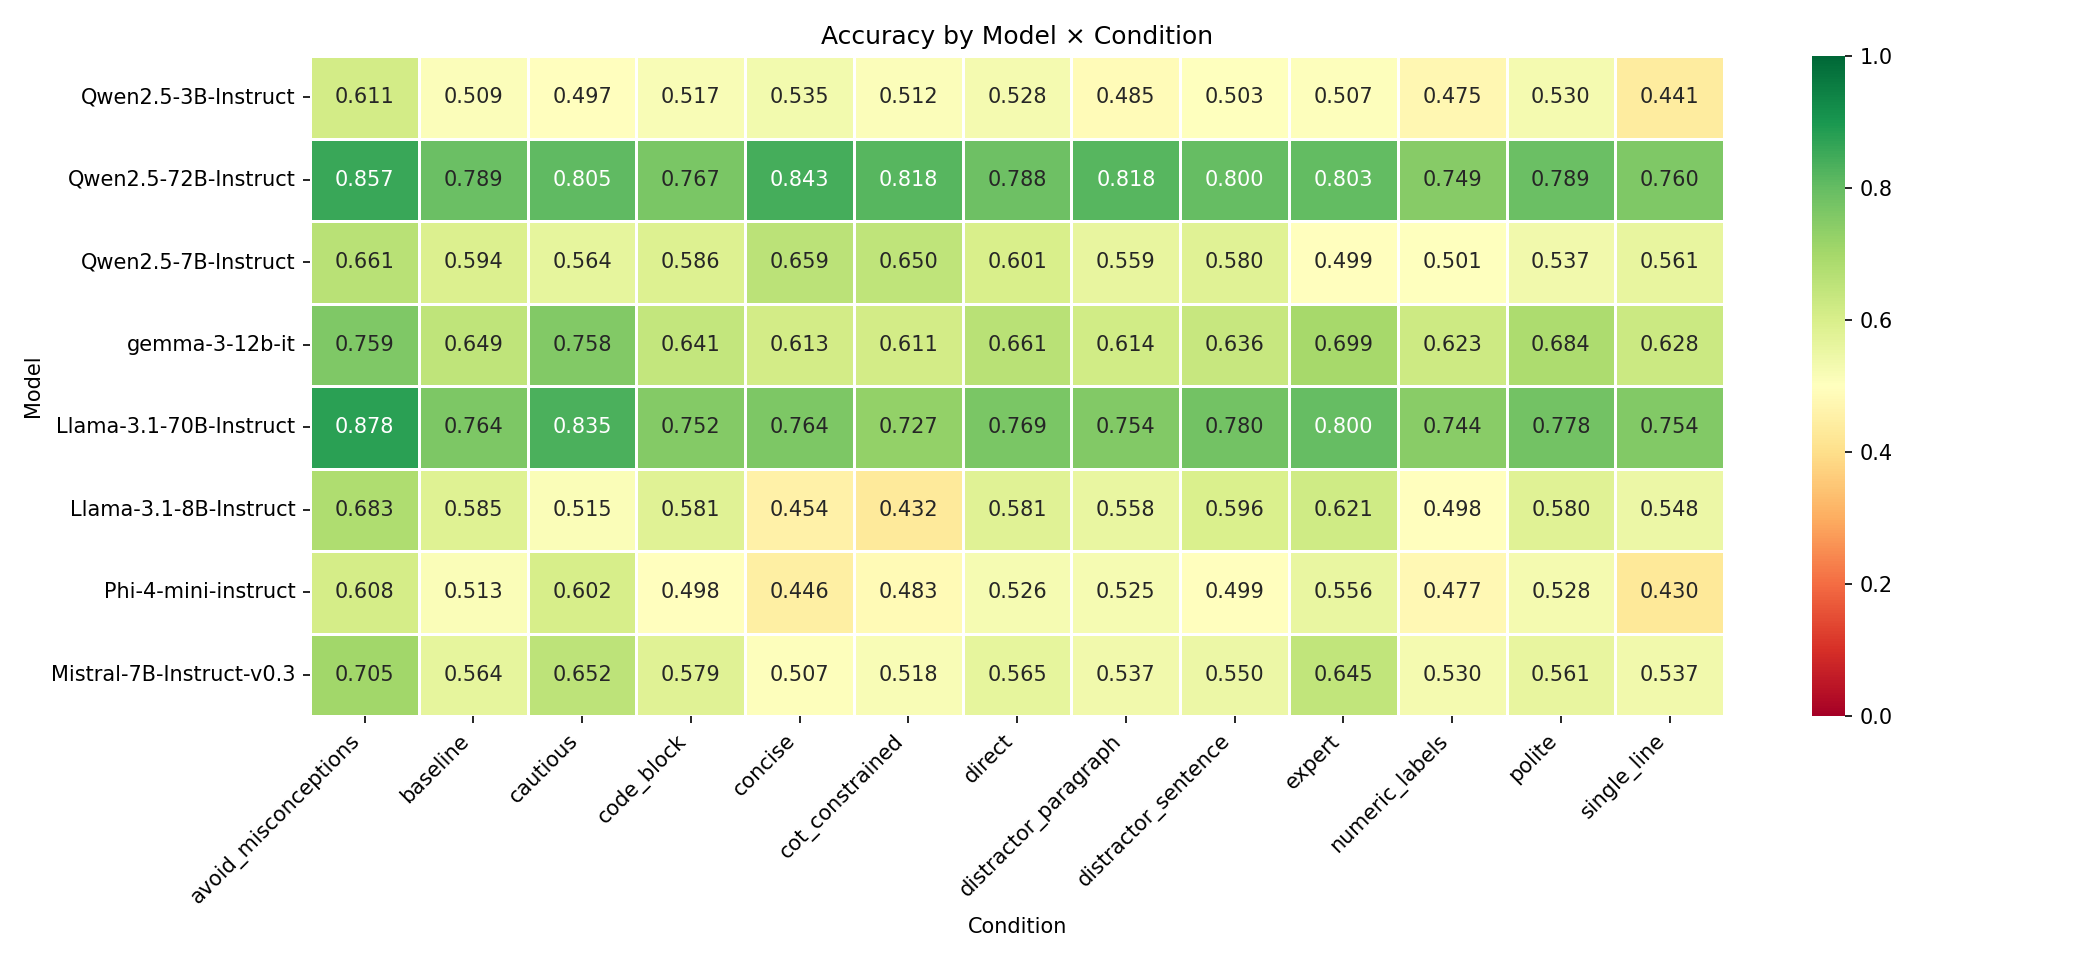
\includegraphics[width=\textwidth]{figures/accuracy_heatmap.png}
\caption{Accuracy heatmap across 8 models (rows) and 13 prompt conditions (columns). Color scale ranges from 0 (red) to 1 (green). \result{Add interpretation.}}
\label{fig:heatmap}
\end{figure}

\subsection{Perturbation Category Analysis}
\label{sec:category}

To understand which types of prompt changes are most disruptive, we group the 12 perturbations by category and compute the mean accuracy delta (relative to baseline) within each group.

\result{Report findings per category. Expected structure:}

\begin{itemize}[leftmargin=*]
    \item \textbf{Instruction wording} (4 conditions): \result{Mean delta = $\pm$XX.X pp.  Which instruction is most harmful? Does ``avoid misconceptions'' help or hurt?}
    \item \textbf{Formatting} (3 conditions): \result{Mean delta.  Does numeric labeling vs.\ alpha labeling matter?  Does single-line layout hurt more than code block?}
    \item \textbf{Benign distractors} (2 conditions): \result{Mean delta.  Does paragraph-length distractor cause more degradation than a single sentence?}
    \item \textbf{Social style} (2 conditions): \result{Mean delta.  Does politeness vs.\ directness matter?}
    \item \textbf{Stress} (1 condition): \result{Delta for CoT-constrained.  Does asking models to ``think step by step'' but output only a label help or hurt?}
\end{itemize}

\result{Are some models disproportionately affected by specific categories?  E.g., do smaller models suffer more from formatting changes?}

\subsection{Ranking Instability}
\label{sec:ranking}

\paragraph{Kendall's $\tval$ by condition.}
Figure~\ref{fig:kendall} plots Kendall's $\tval$ for each condition relative to the baseline ranking.
\result{Which conditions cause the most ranking disruption ($\tval$ closest to 0 or negative)?
Is the overall pattern of high or low ranking stability?}

\begin{figure}[t]
\centering
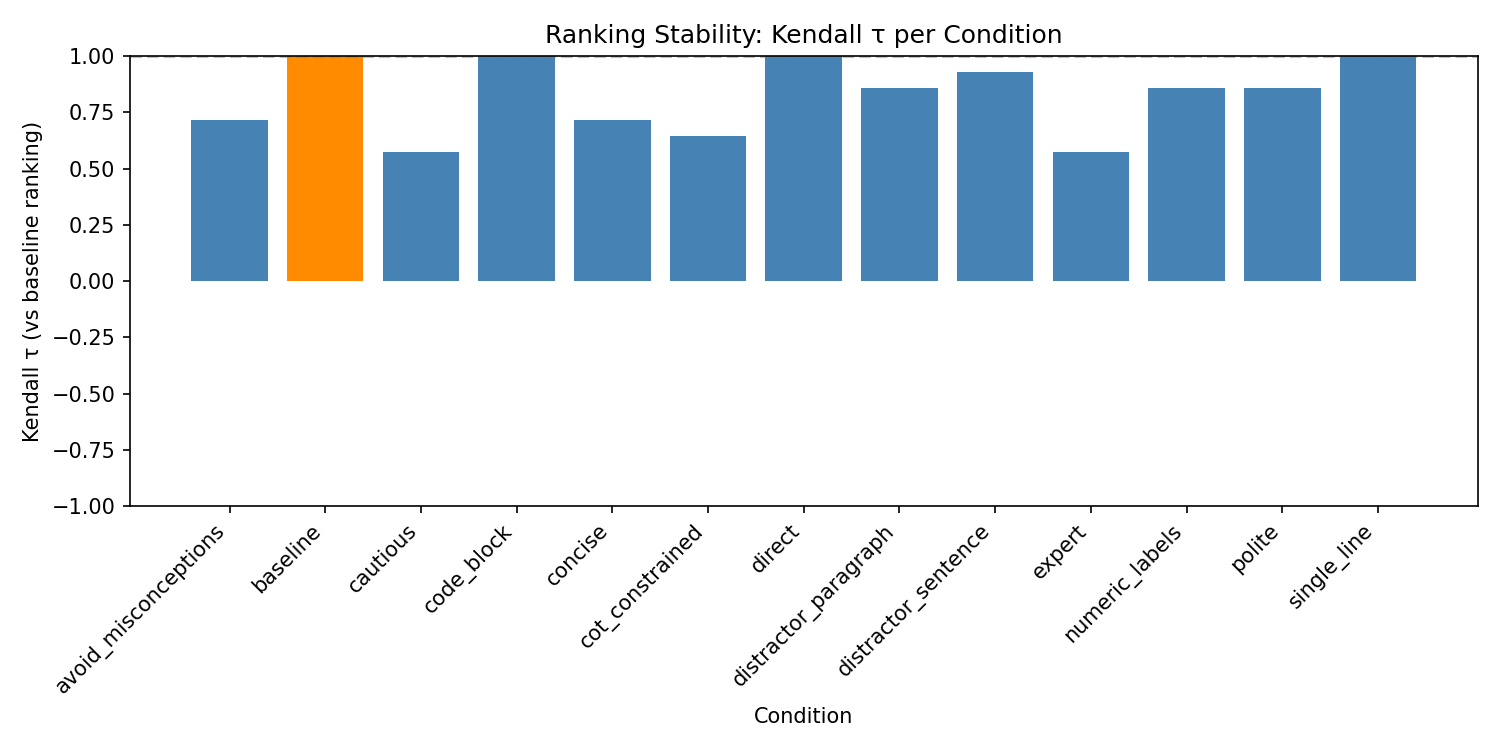
\includegraphics[width=0.85\textwidth]{figures/kendall_tau.png}
\caption{Kendall's $\tval$ between baseline and per-condition model rankings. A value of 1.0 indicates identical rankings; lower values indicate greater ranking instability.}
\label{fig:kendall}
\end{figure}

\paragraph{Rank flips and top-1 instability.}
\result{Report overall rank flip rate (e.g., ``X\% of model-pair comparisons flip across conditions'').}
\result{Report top-1 instability (e.g., ``The top-ranked model changes in Y out of 13 conditions'').}

\paragraph{Baseline vs.\ worst-case scatter.}
Figure~\ref{fig:scatter} plots each model's baseline accuracy against its worst-case accuracy.
Points below the diagonal indicate models that experience accuracy drops under some prompt condition.
\result{Are all points below the diagonal?  Which model has the largest gap (highest PSI)?  Do larger models cluster closer to the diagonal?}

\begin{figure}[t]
\centering
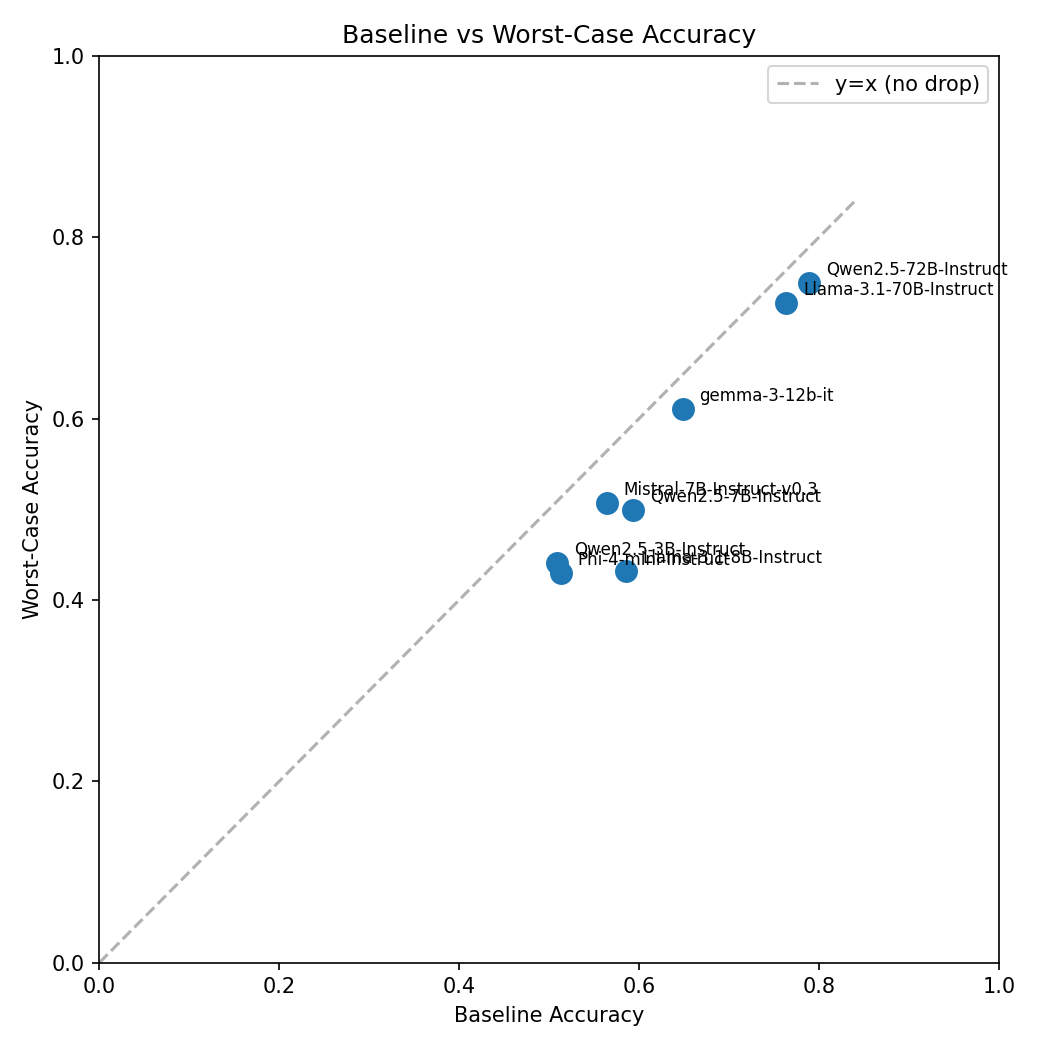
\includegraphics[width=0.6\textwidth]{figures/baseline_vs_worst.png}
\caption{Baseline accuracy vs.\ worst-case accuracy across prompt conditions. Distance below the $y = x$ diagonal equals PSI.}
\label{fig:scatter}
\end{figure}

\subsection{Statistical Significance}
\label{sec:significance}

Table~\ref{tab:bootstrap} summarizes the paired bootstrap results.
For each model, we report the number of conditions (out of 12 perturbations) where the accuracy delta's 95\% CI excludes zero.

\result{How many (model, condition) pairs show statistically significant deltas?
Do significant drops cluster in particular categories?
Are any conditions associated with significant \emph{improvements} over baseline?}

\begin{table}[t]
\centering
\caption{Paired bootstrap summary. For each model, we report the number of perturbation conditions (out of 12) with statistically significant accuracy deltas (95\% CI excludes zero), along with the most negative and most positive observed deltas.}
\label{tab:bootstrap}
\small
\begin{tabular}{@{}lccc@{}}
\toprule
\textbf{Model} & \textbf{Sig.\ conditions} & \textbf{Worst $\delta$} & \textbf{Best $\delta$} \\
\midrule
Qwen2.5-3B      & \result{--} & \result{--} & \result{--} \\
Qwen2.5-7B      & \result{--} & \result{--} & \result{--} \\
Qwen2.5-72B     & \result{--} & \result{--} & \result{--} \\
Llama-3.1-8B    & \result{--} & \result{--} & \result{--} \\
Llama-3.1-70B   & \result{--} & \result{--} & \result{--} \\
Mistral-7B-v0.3 & \result{--} & \result{--} & \result{--} \\
Gemma-3-12B     & \result{--} & \result{--} & \result{--} \\
Phi-4-mini      & \result{--} & \result{--} & \result{--} \\
\bottomrule
\end{tabular}
\end{table}


% ============================================================================
% 5. ANALYSIS
% ============================================================================
\section{Analysis}
\label{sec:analysis}

\subsection{Does Scale Reduce Prompt Fragility?}
\label{sec:scale}

Our model selection allows within-family scaling comparisons: Qwen~2.5 at 3B, 7B, and 72B, and Llama~3.1 at 8B and 70B.

\result{Report PSI trend across scales within each family.  Does the 72B Qwen model have lower PSI than the 3B?  Does Llama-70B have lower PSI than Llama-8B?}

\result{Also report whether the \emph{type} of fragility changes with scale (e.g., smaller models fail more on formatting, larger models are more sensitive to instruction wording).}

Prior work presents mixed evidence on the relationship between scale and robustness.
\citet{sclar2024quantifying} found that scaling alone does not eliminate format sensitivity, while \citet{wang2024prosa} reported a general trend toward greater robustness at larger scales but with substantial task-dependent variation.
\result{How do our findings align with or challenge these prior results?}

\subsection{Cross-Family Comparison at Similar Scale}
\label{sec:crossfamily}

At the 7--12B scale, we compare Qwen~2.5-7B, Llama~3.1-8B, Mistral-7B-v0.3, and Gemma~3-12B.
These models have comparable parameter counts but differ in training data, instruction-tuning procedures, and architectural details.

\result{Which model is most/least robust at this scale?  Are there consistent patterns (e.g., one model is robust to formatting but fragile to instruction wording)?}

\result{Does Phi-4-mini (3.8B, ``small-but-strong'') achieve robustness comparable to larger models?}

\subsection{Invalid Response Rates}
\label{sec:invalid}

A model's inability to produce a parseable answer label is itself an indicator of prompt sensitivity.
\result{Report invalid rates by model and condition.  Are certain conditions associated with high invalid rates (e.g., code\_block, cot\_constrained)?  Do invalid rates correlate with model scale?}


% ============================================================================
% 6. DISCUSSION
% ============================================================================
\section{Discussion}
\label{sec:discussion}

\paragraph{Benchmark scores are distributions, not point estimates.}
Our results demonstrate that TruthfulQA MC1 accuracy varies non-trivially under benign prompt perturbations.
\result{Summarize the magnitude: ``PSI values range from X to Y percentage points, meaning that...''}
This has direct practical implications: a model's reported TruthfulQA score depends not only on its knowledge and reasoning capabilities but also on the specific prompt used to elicit answers.
Two researchers evaluating the same model with different---but equally reasonable---prompt formulations could arrive at meaningfully different accuracy estimates.

\paragraph{Rankings are not stable.}
\result{Summarize ranking instability findings.}
The fact that the ``best'' model can change depending on prompt formulation challenges the practice of comparing models via single-point leaderboard entries.
This is particularly concerning in deployment contexts where model selection decisions have real-world consequences (e.g., medical or legal question answering).

\paragraph{Recommendations for benchmark reporting.}
Based on our findings, we recommend:
\begin{enumerate}[leftmargin=*]
    \item \textbf{Report sensitivity ranges.} When publishing benchmark results, report accuracy under at least 3--5 prompt variants in addition to the primary score, and include PSI or a similar spread metric.
    \item \textbf{Standardize prompt templates.} Cross-model comparisons should use identical prompt templates. When this is not possible (e.g., when models require different chat templates), the prompt-induced variance should be explicitly acknowledged and quantified.
    \item \textbf{Distinguish robustness from accuracy.} A model with slightly lower baseline accuracy but much lower PSI may be preferable in applications where consistent performance matters more than peak performance.
    \item \textbf{Include invalid rates.} Reporting only accuracy ignores cases where the model fails to produce a parseable response. Invalid rates provide complementary information about a model's ability to follow formatting instructions.
\end{enumerate}

\paragraph{Limitations.}
Several limitations of our study should be noted:
\begin{itemize}[leftmargin=*]
    \item \textbf{Model selection.} We evaluate 8 models from 5 families. While this spans a wide range of scales and architectures, it does not cover all major model families (e.g., Claude, GPT, Command R) or very recent releases.
    \item \textbf{Single benchmark.} Our findings are specific to TruthfulQA MC1. The magnitude and pattern of prompt sensitivity may differ for other benchmarks (MMLU, ARC, HellaSwag) or other TruthfulQA configurations (MC2, open-ended).
    \item \textbf{English only.} All experiments are conducted in English. Prompt sensitivity may be amplified or attenuated in other languages.
    \item \textbf{Hand-crafted perturbations.} Our 13 conditions, while spanning 5 categories, are not exhaustive. A larger or automatically generated perturbation set might reveal additional sensitivity patterns.
    \item \textbf{Deterministic decoding.} We use greedy decoding throughout. Sampling-based decoding would introduce additional variance, potentially interacting with prompt sensitivity in complex ways.
    \item \textbf{MC format only.} Multiple-choice evaluation constrains the output space and may underestimate prompt sensitivity compared to open-ended generation, where output format is unconstrained.
\end{itemize}


% ============================================================================
% 7. CONCLUSION
% ============================================================================
\section{Conclusion}
\label{sec:conclusion}

We have presented a systematic evaluation of prompt sensitivity in TruthfulQA multiple-choice scoring across eight instruction-tuned LLMs.
Our key findings are:

\begin{enumerate}[leftmargin=*]
    \item \textbf{Benign prompt changes cause non-trivial accuracy variation.} \result{PSI values range from X to Y pp, with an average of Z pp across models.}
    \item \textbf{Model rankings are \result{stable/unstable} under prompt perturbations.} \result{Kendall's $\tval$ averages W across conditions; the top-ranked model changes in V out of 13 conditions.}
    \item \textbf{Perturbation categories differ in impact.} \result{Category X causes the largest drops on average, while category Y has minimal effect.}
    \item \textbf{Scale provides \result{partial/limited/no} protection.} \result{Within both the Qwen and Llama families, larger models show [lower/similar/higher] PSI.}
\end{enumerate}

The Prompt Sensitivity Index provides a simple, actionable metric for quantifying how much a model's benchmark score depends on prompt formulation.
We recommend that future benchmark evaluations report PSI (or analogous spread metrics) alongside point accuracy estimates, and that model comparisons explicitly account for prompt-induced measurement uncertainty.

Our evaluation framework, all 13 prompt conditions, and complete per-prediction logs are publicly available to facilitate reproducible prompt sensitivity auditing across other benchmarks and model families.


% ============================================================================
% BROADER IMPACT
% ============================================================================
\section*{Broader Impact}
\label{sec:impact}

This work investigates the reliability of a widely used LLM evaluation benchmark.
Our findings have several implications for the broader AI community:

\paragraph{Positive impacts.}
By quantifying how much benchmark scores depend on prompt formulation, our work encourages more rigorous evaluation practices.
If adopted, reporting sensitivity ranges alongside point estimates would give practitioners a more honest picture of model capabilities, leading to better-informed deployment decisions.
This is particularly important in high-stakes domains (healthcare, legal, finance) where model selection based on misleading benchmarks could have real-world consequences.

Our PSI metric is intentionally simple and requires no additional infrastructure beyond running the same evaluation with a few prompt variants.
This low barrier to adoption increases the likelihood that sensitivity reporting becomes standard practice.

\paragraph{Potential negative impacts.}
One concern is that our findings could be used to ``game'' benchmarks---i.e., to select the prompt variant that maximizes a model's score on a particular benchmark.
However, we argue that this risk already exists (and is arguably already exploited) in the current single-prompt paradigm, where the choice of prompt template is often not well-justified.
Making prompt sensitivity explicit and measurable reduces, rather than increases, the scope for gaming, because it shifts the evaluation norm from ``report the best number'' to ``report the range.''

Another concern is that highlighting benchmark fragility might undermine trust in LLM evaluations more broadly.
We view this as a necessary corrective rather than a harm: trust in evaluation should be calibrated to the actual reliability of the measurements, and our results suggest that current practice overstates precision.

\paragraph{Environmental impact.}
Running 8 models $\times$ 13 conditions $\times$ 736 questions requires approximately \result{XX GPU-hours} on NVIDIA H200 GPUs.
While not negligible, this is modest compared to model training costs, and the reusable framework amortizes this cost across future evaluations.

\paragraph{Data and ethical considerations.}
TruthfulQA contains questions about sensitive topics (health, law, conspiracy theories).
Our study does not generate novel misinformation; it evaluates models' ability to select correct answers from pre-existing options.
All evaluation is automated with no human subjects.


% ============================================================================
% REFERENCES
% ============================================================================
\bibliographystyle{plainnat}
% \bibliography{references}  % uncomment when references.bib is ready

\begin{thebibliography}{20}

\bibitem[Alzahrani et~al.(2024)]{alzahrani2024benchmarks}
Norah Alzahrani, Hisham Alyahya, et~al.
\newblock When benchmarks are targets: Revealing the sensitivity of large language model leaderboards.
\newblock In \emph{Proceedings of the 62nd Annual Meeting of the Association for Computational Linguistics}, 2024.

\bibitem[Hendrycks et~al.(2021)]{hendrycks2021measuring}
Dan Hendrycks, Collin Burns, Steven Basart, Andy Zou, Mantas Mazeika, Dawn Song, and Jacob Steinhardt.
\newblock Measuring massive multitask language understanding.
\newblock In \emph{Proceedings of ICLR}, 2021.

\bibitem[Lin et~al.(2022)]{lin2022truthfulqa}
Stephanie Lin, Jacob Hilton, and Owain Evans.
\newblock TruthfulQA: Measuring how models mimic human falsehoods.
\newblock In \emph{Proceedings of the 60th Annual Meeting of the Association for Computational Linguistics}, pages 3214--3252, 2022.

\bibitem[Mizrahi et~al.(2024)]{mizrahi2024state}
Moran Mizrahi, Guy Kaplan, Dan Malkin, Rotem Dror, Dafna Shahaf, and Gabriel Stanovsky.
\newblock State of what art? {A} call for multi-prompt {LLM} evaluation.
\newblock \emph{Transactions of the Association for Computational Linguistics}, 12:933--949, 2024.

\bibitem[Polo et~al.(2024)]{polo2024tinybenchmarks}
Felipe~Maia Polo, Lucas Weber, Leshem Choshen, Yuekai Sun, Gongjun Xu, and Mikhail Yurochkin.
\newblock tinyBenchmarks: evaluating {LLMs} with fewer examples.
\newblock In \emph{Proceedings of ICML}, 2024.

\bibitem[Ronacher(2008)]{ronacher2008jinja2}
Armin Ronacher.
\newblock Jinja2 documentation.
\newblock \url{https://jinja.palletsprojects.com/}, 2008.

\bibitem[Sclar et~al.(2024)]{sclar2024quantifying}
Melanie Sclar, Yejin Choi, Yulia Tsvetkov, and Alane Suhr.
\newblock Quantifying language models' sensitivity to spurious features in prompt design, or: How {I} learned to start worrying about prompt formatting.
\newblock In \emph{Proceedings of ICLR}, 2024.

\bibitem[Voronov et~al.(2024)]{voronov2024mind}
Anton Voronov, Lena Wolf, and Max Ryabinin.
\newblock Mind your format: Towards consistent evaluation of in-context learning improvements.
\newblock \emph{arXiv preprint arXiv:2401.06766}, 2024.

\bibitem[Wang et~al.(2024)]{wang2024prosa}
Junda Wang, Xintong Wang, et~al.
\newblock {ProSA}: Assessing and understanding the prompt sensitivity of {LLMs}.
\newblock In \emph{Findings of EMNLP}, 2024.

\bibitem[Zellers et~al.(2019)]{zellers2019hellaswag}
Rowan Zellers, Ari Holtzman, Yonatan Bisk, Ali Farhadi, and Yejin Choi.
\newblock HellaSwag: Can a machine really finish your sentence?
\newblock In \emph{Proceedings of the 57th Annual Meeting of the Association for Computational Linguistics}, 2019.

\bibitem[Zheng et~al.(2024)]{zheng2024prompt}
Lianghui Zheng, Aobo Wang, et~al.
\newblock Judging {LLM}-as-a-judge with {MT-Bench} and Chatbot Arena.
\newblock In \emph{Advances in Neural Information Processing Systems}, 2024.

\bibitem[Zhu et~al.(2023)]{zhu2023promptrobust}
Kaijie Zhu, Jindong Wang, Jiaheng Zhou, Zichen Wang, Hao Chen, Yidong Wang, Linyi Yang, Wei Ye, Yue Zhang, Neil~Zhenqiang Gong, and Xing Xie.
\newblock {PromptRobust}: Towards evaluating the robustness of large language models on adversarial prompts.
\newblock \emph{arXiv preprint arXiv:2306.04528}, 2023.

\bibitem[Zhu et~al.(2024)]{zhu2024benchbench}
Yotam Zhu, et~al.
\newblock {BenchBench}: Meta-evaluation for {AI} benchmarks.
\newblock \emph{arXiv preprint}, 2024.

\end{thebibliography}


% ============================================================================
% APPENDIX
% ============================================================================
\newpage
\appendix

\section{Full Prompt Text for All 13 Conditions}
\label{app:prompts}

For reproducibility, we provide the exact rendered prompt for an example question under each of the 13 conditions.
All conditions use the same Jinja2 template with different parameter values.

\result{Generate an example question rendered under all 13 conditions after results are available. Include the full prompt text for each condition.}

\section{Per-Question Sensitivity Breakdown}
\label{app:perquestion}

\result{Analyze which questions are most sensitive to prompt variation. Report the distribution of per-question accuracy ranges across conditions. Are there ``fragile questions'' that all models get wrong under certain conditions but right under others?}

\section{Detailed Bootstrap Delta Tables}
\label{app:bootstrap}

\result{Full table of observed deltas and 95\% CIs for all (model $\times$ condition) pairs. Mark significant entries with *.}

\section{Computational Resources}
\label{app:compute}

All experiments were conducted on NVIDIA H200 GPUs (80GB HBM3e) using the NVWulf computing cluster.
Models $\leq$12B were run on a single GPU; 70B+ models used multi-GPU inference via HuggingFace Accelerate with \texttt{device\_map="auto"}.

Software versions:
\begin{itemize}[leftmargin=*]
    \item Python 3.11
    \item PyTorch $\geq$ 2.1.0
    \item Transformers $\geq$ 4.46.0, $<$ 5.0.0
    \item CUDA 12.8
\end{itemize}

Total wall-clock time for all 8 models $\times$ 13 conditions: \result{XX hours on 1$\times$ H200.}

\end{document}
